% BHU PYQ -- Professional Exam Template
\documentclass[11pt,a4paper]{article}

\usepackage[a4paper,top=2.5cm,bottom=2.5cm,left=2.8cm,right=2.8cm,headheight=14pt]{geometry}
\usepackage{amsmath,amssymb}
\usepackage[T1]{fontenc}
\usepackage[utf8]{inputenc}
\usepackage{lmodern}
\usepackage{microtype}
\usepackage{fancyhdr}
\usepackage{enumitem}
\usepackage{listings}
\usepackage{tikz}
\usepackage{hyperref}
\usepackage{lastpage}
\usepackage{parskip}

\hypersetup{colorlinks=true,urlcolor=black,linkcolor=black,
  pdftitle={GEN-402: Data Structures Algorithms -- BHU PYQ}}

\pagestyle{fancy}
\fancyhf{}
\renewcommand{\headrulewidth}{0.4pt}
\renewcommand{\footrulewidth}{0.4pt}
\fancyhead[L]{\small\textit{Banaras Hindu University}}
\fancyhead[R]{\small\textit{GEN-402: Data Structures Algorithms}}
\fancyfoot[C]{\small Page \thepage\ of \pageref{LastPage}}

\lstset{
  basicstyle=\small\ttfamily,
  frame=single,
  breaklines=true,
  columns=flexible,
  keepspaces=true
}

\newlist{parts}{enumerate}{2}
\setlist[parts,1]{label=(\alph*),leftmargin=*,itemsep=4pt,topsep=3pt}
\setlist[parts,2]{label=(\roman*),leftmargin=*,itemsep=2pt,topsep=2pt}
\newcommand{\pts}[1]{\hfill\textit{[#1]}}

\begin{document}

\begin{center}
  {\large\bfseries BANARAS HINDU UNIVERSITY}\\[2pt]
  {\normalsize B.Voc. Semester IV Examination, 2022-23}\\[6pt]
  \rule{0.8\linewidth}{0.5pt}\\[6pt]
  {\large\bfseries Paper: GEN-402 --- Data Structures Algorithms}\\[4pt]
  {\normalsize Time: Three hours \hfill Maximum Marks: 70}
\end{center}

\rule{\linewidth}{0.4pt}

\smallskip
\noindent\textit{Instructions: Attempt all questions. Symbols have their usual meanings.}

\bigskip

\noindent{\large\bfseries SECTION --- A}\\[4pt]
\rule{\linewidth}{0.4pt}\smallskip

Long-Answer Questions. Answer any two questions: \hfill \textbf{2 $\times$ 12 = 24 Marks}

\medskip
\noindent\textbf{Question 1.} Define Linked Lists. What are the basic operations performed on a Linked List? Write methods for the creation of a Linked List and insertion of any three elements at the beginning of the list.

\medskip
\noindent\textbf{Question 2.} What is a Binary Tree? Explain Preorder, Inorder, and Postorder traversals of a binary tree with suitable examples.

\medskip
\noindent\textbf{Question 3.} What is a Graph data structure? Explain the Breadth First Search (BFS) algorithm with a suitable example. Differentiate between Breadth First Search and Depth First Search.

\medskip
\noindent\textbf{Question 4.} Explain Stack Data Structure. Write a program to implement a stack using an array (show creation, insertion, deletion, and display of elements).

\bigskip\noindent{\large\bfseries SECTION --- B}\\[4pt]
\rule{\linewidth}{0.4pt}\smallskip

Attempt any six questions: \hfill \textbf{6 $\times$ 6 = 36 Marks}

\medskip
\noindent\textbf{Question 5.} Explain Binary Search with a suitable example. What is the prerequisite condition to implement binary search?

\medskip
\noindent\textbf{Question 6.} Explain Prim's algorithm to find a Minimum Spanning Tree (MST). Find the cost of the minimum spanning tree of the following graph:
\begin{center}
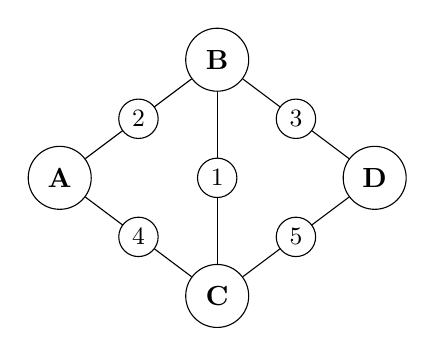
\begin{tikzpicture}[>=stealth,
  state/.style={draw, circle, minimum size=8mm, inner sep=0pt, font=\bfseries},
  weight/.style={draw, circle, fill=white, minimum size=5mm, inner sep=0pt, font=\small}
]
  \node[state] (A) at (0,1.5) {A};
  \node[state] (B) at (2,3) {B};
  \node[state] (C) at (2,0) {C};
  \node[state] (D) at (4,1.5) {D};
  
  \draw[-] (A) -- node[weight] {2} (B);
  \draw[-] (A) -- node[weight] {4} (C);
  \draw[-] (B) -- node[weight] {1} (C);
  \draw[-] (B) -- node[weight] {3} (D);
  \draw[-] (C) -- node[weight] {5} (D);
\end{tikzpicture}
\end{center}

\medskip
\noindent\textbf{Question 7.} Explain Bubble Sort with a suitable example.

\medskip
\noindent\textbf{Question 8.} What is recursion? Write a program to find the factorial of a given number using recursion.

\medskip
\noindent\textbf{Question 9.} Explain Insertion Sort using a suitable example.

\medskip
\noindent\textbf{Question 10.} Give the algorithm to evaluate a postfix expression using a stack. Evaluate the postfix expression $5\ 2\ 4\ * + 7\ -$ using the algorithm and show the stack contents at each step.

\medskip
\noindent\textbf{Question 11.} What is an AVL tree? Explain LL and LR rotations.

\medskip
\noindent\textbf{Question 12.} Define a queue data structure. Explain the operations enqueue and dequeue in a queue.

\medskip
\noindent\textbf{Question 13.} Write a Java program to find the minimum and maximum elements in an array of 20 elements. (The elements must be input by the user).

\bigskip\noindent{\large\bfseries SECTION --- C}\\[4pt]
\rule{\linewidth}{0.4pt}\smallskip

\noindent\textbf{Question 14.} Attempt all parts: \hfill \textbf{10 $\times$ 1 = 10 Marks}
\begin{parts}
  \item A Binary Search Tree (BST) has the property that the value of each node in the left subtree is \_\_\_\_\_\_ the value of the root node, and the value of each node in the right subtree is \_\_\_\_\_\_ the value of the root node.
  \begin{enumerate}[label=(\alph*),itemsep=2pt]
    \item Greater, Greater
    \item Greater, Less
    \item Less, Less
    \item Less, Greater
  \end{enumerate}
  
  \item In a stack, which operation is used to remove an element from the stack?
  \begin{enumerate}[label=(\alph*),itemsep=2pt]
    \item Pop
    \item Push
    \item Peek
    \item Empty
  \end{enumerate}
  
  \item Which of the following data structures is not a linear data structure?
  \begin{enumerate}[label=(\alph*),itemsep=2pt]
    \item Stack
    \item Queue
    \item Linked List
    \item Binary Tree
  \end{enumerate}
  
  \item Which of the following data structures finds its use in recursion?
  \begin{enumerate}[label=(\alph*),itemsep=2pt]
    \item Stack
    \item Array
    \item Linked List
    \item Queue
  \end{enumerate}
  
  \item Which of the following is a Divide and Conquer algorithm?
  \begin{enumerate}[label=(\alph*),itemsep=2pt]
    \item Bubble Sort
    \item Selection Sort
    \item Heap Sort
    \item Merge Sort
  \end{enumerate}
  
  \item Which data structure is needed to convert infix notation to postfix notation?
  \begin{enumerate}[label=(\alph*),itemsep=2pt]
    \item Tree
    \item Graph
    \item Stack
    \item Queue
  \end{enumerate}
  
  \item Evaluate the postfix expression $ab + cd / -$ where $a=5$, $b=4$, $c=9$, $d=3$.
  \begin{enumerate}[label=(\alph*),itemsep=2pt]
    \item 23
    \item 15
    \item 6
    \item 10
  \end{enumerate}
  
  \item The optimal data structure used to solve the Tower of Hanoi is \_\_\_\_\_\_.
  \begin{enumerate}[label=(\alph*),itemsep=2pt]
    \item Tree
    \item Heap
    \item Priority Queue
    \item Stack
  \end{enumerate}
  
  \item What is a linear data structure with FIFO behavior? (Answer in one word).
  
  \item What is the time complexity of Merge Sort? (Answer in one word).
\end{parts}

\vfill
\rule{\linewidth}{0.4pt}
\begin{center}\small
\href{https://bhu-exam.vercel.app/}{Click here to visit our website}\\[4pt]\href{https://me-aryan.vercel.app/}{Click here to visit our contributor}\\[4pt]\href{https://quashan-me.vercel.app/}{Click here to visit our contributor}
\end{center}

\end{document}
